\section{Conceptual Design}
\subsection{Requirements}
The requirements for the database are the following:\begin{table}[H]
    \renewcommand{\arraystretch}{1.3} % Adjust row height
    \begin{tabularx}{\textwidth}{|X|}
    \hline
    \multicolumn{1}{|c|}{\textbf{"GreenWorld Energy"}} \\ \hline
    The company "GreenWorld Energy" operates decentralized renewable energy production facilities distributed 
    across regions. Each facility is characterized by a name, location, type of energy produced (e.g., solar, wind, 
    hydro), and maximum energy output capacity. The company also manages contracts with customers for energy 
    supply, categorized as residential or commercial, and offers flexible pricing models based on consumption. 
    Each customer has one or more accounts, each identified by a unique code. Every energy contract is linked to a 
    single customer account and includes details such as start date, duration, energy plan, and cost. Facilities are 
    overseen by management teams, each identified by a unique code, team name, and the number of projects managed. 
    Teams are evaluated based on performance metrics such as energy efficiency, uptime, and customer satisfaction. 
    Each team is represented by the main responsible employee and other employees identified by fiscal code, name, 
    surname, date of birth and date of hiring. Additionally, the company supports a feedback system allowing 
    customers to submit ratings and comments regarding service quality. Customers are classified into residential and 
    commercial types, each identified by a unique alphanumeric code, with associated contact details and energy 
    consumption history. \\ \hline
    \end{tabularx}
    \caption{Requirements}
\end{table}


\subsection{Analysis}

\subsubsection{Reorganization of Concepts}
The concepts can be reorganized as follows:
\begin{table}[H]
    \renewcommand{\arraystretch}{1.3} % Adjust row height
    \begin{tabularx}{\textwidth}{|X|}
    \hline  \multicolumn{1}{|c|}{\textbf{Facility}}    \\ \hline
    Each facility is characterized by a name, location, type of energy produced (e.g., solar, wind, hydro), and maximum energy output capacity. The company also manages contracts with customers for energy supply, categorized as residential or commercial, and offers flexible pricing models based on consumption. Facilities are overseen by management teams \\ \hline
    \end{tabularx}
    \caption{Facility's Concepts}
    \end{table}

\begin{table}[H]
    \renewcommand{\arraystretch}{1.3} % Adjust row height
    \begin{tabularx}{\textwidth}{|X|}
    \hline  \multicolumn{1}{|c|}{\textbf{Contract}}    \\ \hline
    The company also manages contracts with customers for energy supply, categorized as residential or commercial, and offers flexible pricing models based on consumption.
    Every enegry contract is linked to a single customer account and includes details such as start date, duration, energy plan, and cost. \\ \hline
    \end{tabularx}
    \caption{Contract's Concepts}
    \end{table}

\begin{table}[H]
    \renewcommand{\arraystretch}{1.3} % Adjust row height
    \begin{tabularx}{\textwidth}{|X|}
    \hline  \multicolumn{1}{|c|}{\textbf{Customer}}   \\ \hline
    Each customer has one or more accounts, each identified by a unique code. Customers are classified into residential and commercial types, each identified by a unique alphanumeric code, with associated contact details and energy consumption history. Additionally, the company supports a feedback system allowing customers to submit ratings and comments regarding service quality. \\ \hline
    \end{tabularx}
    \caption{Customer's Concepts}
    \end{table}

\begin{table}[H]
    \renewcommand{\arraystretch}{1.3} % Adjust row height
    \begin{tabularx}{\textwidth}{|X|}
    \hline   \multicolumn{1}{|c|}{\textbf{Account}}    \\ \hline
    Each customer has one or more accounts, each identified by a unique code. Every energy contract is linked to a single customer account and includes details such as start date, duration, energy plan, and cost. \\ \hline
    \end{tabularx}
    \caption{Account's Concepts}
    \end{table}

\begin{table}[H]
    \renewcommand{\arraystretch}{1.3} % Adjust row height
    \begin{tabularx}{\textwidth}{|X|}
    \hline  \multicolumn{1}{|c|}{\textbf{Feedback}}    \\ \hline
    The company supports a feedback system allowing customers to submit ratings and comments regarding service quality. \\ \hline
    \end{tabularx}
    \caption{Feedback's Concepts}
    \end{table}

\begin{table}[H]
    \renewcommand{\arraystretch}{1.3} % Adjust row height
    \begin{tabularx}{\textwidth}{|X|}
    \hline  \multicolumn{1}{|c|}{\textbf{Team}}    \\ \hline
    Facilities are overseen by management teams, each identified by a unique code, team name, and the number of projects managed. Teams are evaluated based on performance metrics such as energy efficiency, uptime, and customer satisfaction. Each team is represented by the main responsible employee \\ \hline
    \end{tabularx}
    \caption{Team's Concepts}
    \end{table}

\begin{table}[H]
    \renewcommand{\arraystretch}{1.3} % Adjust row height
    \begin{tabularx}{\textwidth}{|X|}
    \hline  \multicolumn{1}{|c|}{\textbf{Employee}}    \\ \hline
    Each team is represented by the main responsible employee and other employees identified by fiscal code, name, surname, date of birth and date of hiring. \\ \hline
    \end{tabularx}
    \caption{Employee's Concepts}
\end{table}

These concepts are elegible to be entities in the database. Region is not included in the concepts because it is not a standalone concept. It is a part of the Facility concept. The Facility concept includes the location of the facility. However, it will be included in the Glossary of Term because of a synonym.
    \subsubsection{Glossary of Terms}
    \begin{table}[H]
        \renewcommand{\arraystretch}{1.3} % Adjust row height
        \begin{tabularx}{\textwidth}{|X|X|X|X|}
        \hline
        \textbf{Term}& \textbf{Description}  & \textbf{Connections}    & \textbf{Synonyms}     \\ \hline
        Region      & Area where the facilities are located. & Facility     & Location \\ \hline
        Facility     & Energy production facility. It emits energy for customers      & Contract,Teams,Region         &\\ \hline
        Contract     & Energy supply contract. It describes the energy plan. It can be residential or commercial & Account, Facility     &  Projects        \\ \hline
        Customer     & Customer of GreenWorld Energy. It can be residential or commercial       & Account    &        \\ \hline
        Account      & Customer account. It associated with only one account and one contract & Contract, Customer, Feedback     &        \\ \hline
        Feedback     & Customer feedback. Used to give a score to each team       & Account,Team     &         Ratings, customer satisfaction \\\hline
        Team        & Groups of employees that oversees a facility. Each team has a manager       & Facility, Employee, Feedback     &  Management team       \\ \hline
        Employee     & Employee of a GreenWorld Energy's team.      & Team     &        \\ \hline
        \end{tabularx}
        \caption{Glossary of Terms}
        \end{table}
  
    \subsubsection{Level of Abstraction}
    By considering the synonyms of the terms, we can identify the level of abstraction of the terms. The terms can be classified as follows:
    \begin{itemize}
        \item \textbf{Region} as Location
        \item \textbf{Facility} as Facility
        \item \textbf{Contract} as Contract
        \item \textbf{Customer} as Customer
        \item \textbf{Account} as Account
        \item \textbf{Feedback} as Feedback
        \item \textbf{Team} as Team
        \item \textbf{Employee} as Employee
    \end{itemize}



\subsubsection{Entity-Relationship Diagram}

\paragraph{SKELETON SCHEMA} \leavevmode \newline
\begin{figure}[H]
    \centering
    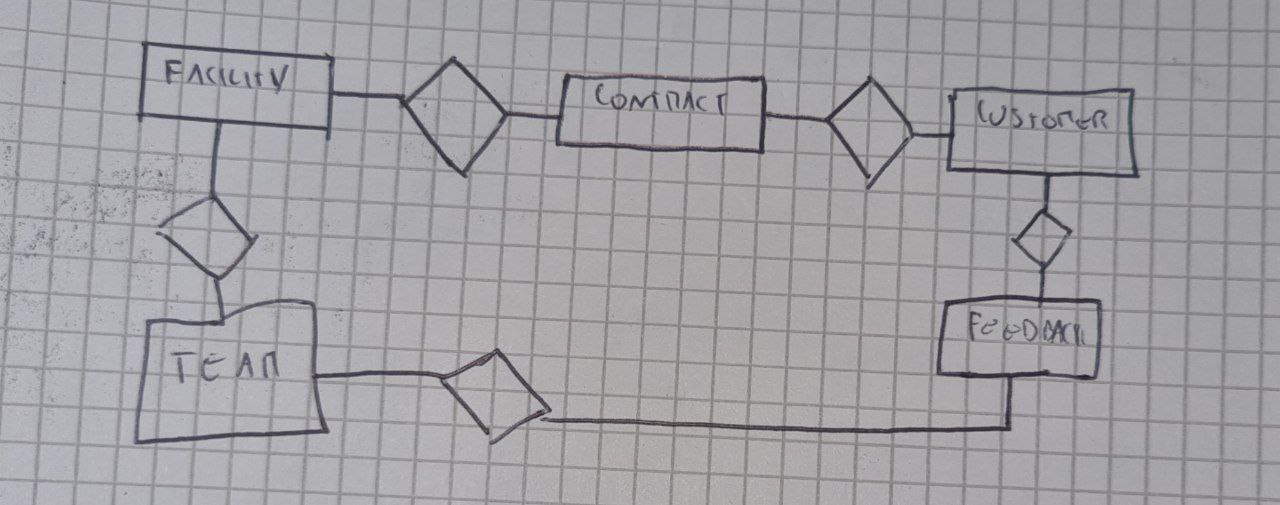
\includegraphics[width=\textwidth]{images/SkeletonSchema.png}
    \caption{Skeleton Schema}
\end{figure}

\noindent This schema represents the main entities and their relationships. The entities are the following:
\begin{itemize}
    \item \textbf{Facility}
    \item \textbf{Contract}
    \item \textbf{Customer}
    \item \textbf{Feedback}
    \item \textbf{Team}
\end{itemize}
The purpose of this schema is to have a general idea of the entities and their relationships. The attributes of the entities and the cardinality of the relationships are not included in this schema. Also, some entities are not included in this schema, such as Account and Employee. These entities will be included in the final schema with all the other details.

\paragraph{FINAL SCHEMA} \leavevmode \newline

\begin{figure}[H]
    \centering
    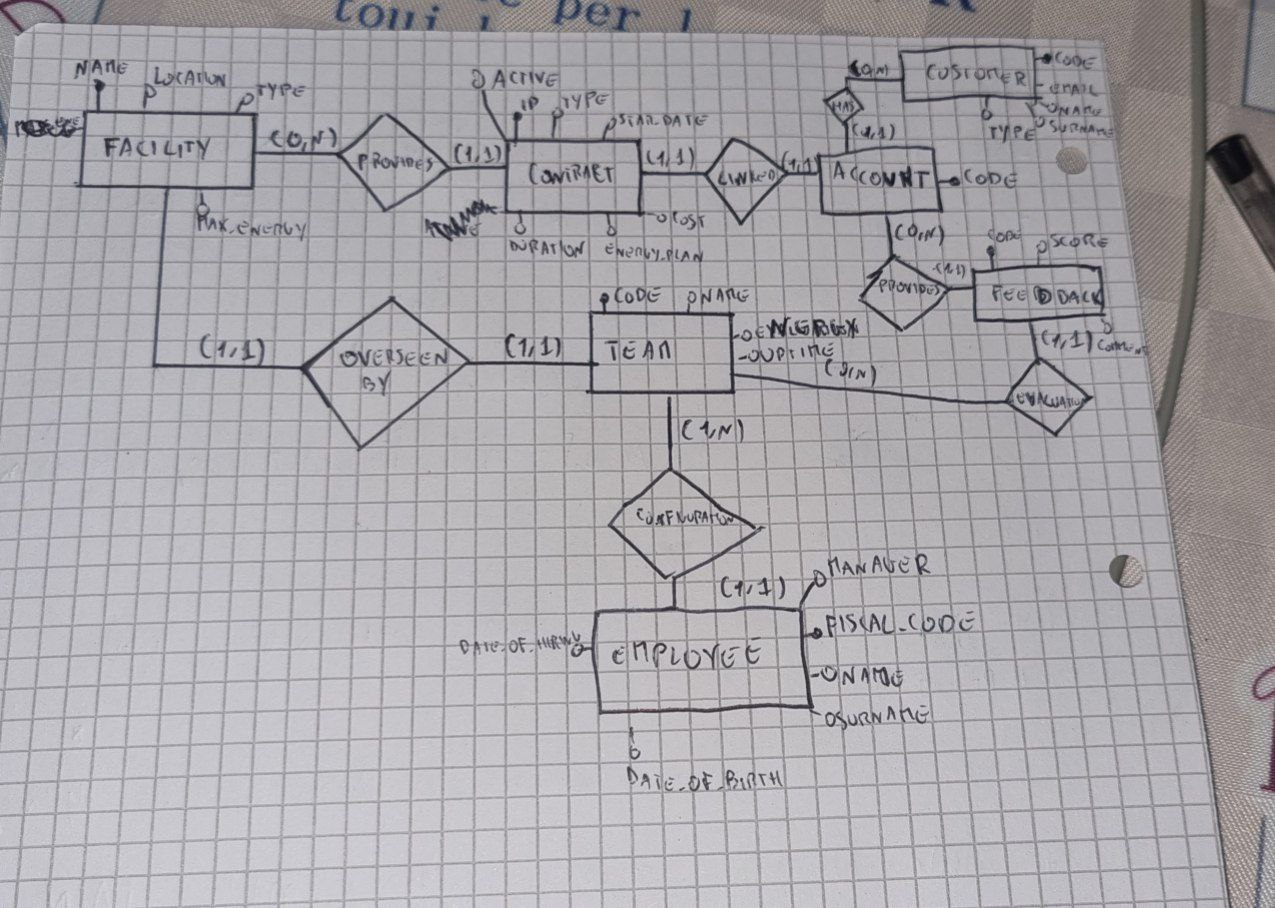
\includegraphics[width=\textwidth]{images/ER.png}
    \caption{Final Schema}
\end{figure}

\noindent Note: Duration is expressed in months

\subsubsection{Business Rules}
The business rules are the following:
\begin{itemize}
    \item A customer can't be a minor
    \item An employee can't be a minor
    \item Each team has got only one main responsible employee
    \item The sum of energy plan of all contracts related to a facility can't exceed the maximum energy output capacity of the facility
    \item If an account needs to activate a new contract with the same facility, the old contract must deactivated before the new one is activated
    \item A customer of a specific type can't have a contract of the other type
    \item The score of a feedback can be between 0 and 5
    \item Uptime is the number of hours the facility is active in a day. Between 6 and 8
    \item Energy efficiency is the percentage of energy produced compared to the maximum energy output capacity of the facility. Between 0 and 100
    \item EnergyPlan can be; 2.500 kWh, 4.500 kWh or 10.000 kWh
    \item Cost: 500 if EnergyPlan=2.500, 750 if EnergyPlan=4.500, 1000 if EnergyPlan=10.000
\end{itemize}



